\chapter{信号分析基础}
\label{chap:hw-signals}

\noindent 本章对应 CH2 作业的6道题，沿用如下傅里叶变换约定：
\[
    X(f)=\int_{-\infty}^{+\infty}x(t)e^{-\iu 2\pi ft}\diff t,
    \qquad \Omega=2\pi f\ \text{（谱角频率）},
    \qquad \Sa z=\frac{\sin z}{z},\quad \Sa 0=1.
\]
符号函数和阶跃函数需要用\textbf{广义傅里叶变换}处理；
普通傅里叶变换则根据全时间轴上的信号定义，选用积分法或性质法。

\needspace{11\baselineskip}
\section{第1题：正弦信号的绝对均值与方均根值}
\label{hw:2-1}
\keypoint{复习重点：周期平均、绝对均值、均方值与方均根值的区别。}

\begin{hwquestion}
求正弦信号 $x(t)=x_0\sin\omega t$ 的绝对均值（原题记作 $|\mu_x|$）和方均根值 $x_{\mathrm{rms}}$。
    设 $\omega>0$，周期为 $T_0=2\pi/\omega$。
\end{hwquestion}

\subsection*{答案与解析}
\textbf{先写定义，再做一个周期的积分。}
绝对均值是信号绝对值在一个周期内的平均值，
方均根值是均方值的平方根。分别定义为
\[
    \mu_{|x|}=\frac{1}{T_0}\int_0^{T_0}|x(t)|\diff t,
    \qquad
    x_{\mathrm{rms}}=
    \sqrt{\frac{1}{T_0}\int_0^{T_0}x^2(t)\diff t}.
\]
令 $\theta=\omega t$，由 $\diff t=\diff\theta/\omega$ 得
\begin{align*}
    \mu_{|x|}
    &=\frac{|x_0|}{2\pi}
      \int_0^{2\pi}|\sin\theta|\diff\theta \\
    &=\frac{|x_0|}{2\pi}
      \left(\int_0^\pi\sin\theta\diff\theta
      -\int_\pi^{2\pi}\sin\theta\diff\theta\right)
      =\boxed{\frac{2|x_0|}{\pi}}.
\end{align*}
用 $\sin^2\theta=(1-\cos2\theta)/2$ 求均方值：
\begin{align*}
    \overline{x^2}
    &=\frac{x_0^2}{2\pi}\int_0^{2\pi}\sin^2\theta\diff\theta
      =\frac{x_0^2}{2}, \\
    x_{\mathrm{rms}}
    &=\sqrt{\overline{x^2}}
      =\boxed{\frac{|x_0|}{\sqrt{2}}}.
\end{align*}
若 $x_0>0$ 表示峰值，可直接写成
$\mu_{|x|}=2x_0/\pi$、$x_{\mathrm{rms}}=x_0/\sqrt{2}$。




\subsection*{本题知识点与公式}
\label{kn:2-1}
\begin{focusbox}{首次学习：周期、信号强度、有效值与能量/功率}
本题没有前置的专业知识块。应掌握“先规定平均区间，再进行整流或平方，最后取平均”的顺序；均值、绝对均值和有效值分别保留不同的信息，不能相互代替。
\end{focusbox}

\subsubsection*{1. 周期、频率与相位分别描述什么}
连续时间信号用 $x(t)$ 描述，$t$ 的单位为秒；连续时间不要求波形处处连续，阶跃也属于连续时间信号。若存在 $T_0>0$ 使 $x(t+T_0)=x(t)$，则为周期信号；最小正周期称基本周期。对非零正弦，
\[
T_0=\frac{2\pi}{\omega},\qquad f_0=\frac1{T_0},\qquad
\omega=2\pi f_0.
\]
$f_0$ 的单位为 Hz，$\omega$ 的单位为 $\mathrm{rad/s}$。$X_p\sin(\omega t+\theta)$ 中 $X_p\geq0$ 是峰值，$\theta$ 是初相位；相位只改变周期内各数值出现的时刻，不改变完整周期平均后的强度。多个正弦叠加能否有共同周期，要检查非零频率之比是否均为有理数，不能任意选某一分量的周期作为整个信号的周期。

\subsubsection*{2. 六个常用时域量及其物理意义}
对实周期信号，在任意完整周期 $[t_*,t_*+T_0]$ 内定义
\begin{align*}
\mu_x&=\frac1{T_0}\int_{t_*}^{t_*+T_0}x(t)\diff t
&&\text{均值，保留正负抵消后的直流分量},\\
\mu_{|x|}&=\frac1{T_0}\int_{t_*}^{t_*+T_0}|x(t)|\diff t
&&\text{绝对均值，也称整流平均值},\\
\psi_x^2&=\frac1{T_0}\int_{t_*}^{t_*+T_0}x^2(t)\diff t
&&\text{均方值},\\
x_{\mathrm{rms}}&=\sqrt{\psi_x^2}
&&\text{方均根值，也称有效值},\\
\sigma_x^2&=\frac1{T_0}\int_{t_*}^{t_*+T_0}[x(t)-\mu_x]^2\diff t
&&\text{去掉直流后的均方波动},\\
x_p&=\max_t|x(t)|,\quad x_{\mathrm{pp}}=x_{\max}-x_{\min}
&&\text{绝对峰值与峰峰值}.
\end{align*}
均值、绝对均值、有效值、标准差 $\sigma_x$ 与 $x$ 同单位；均方值和方差为该单位的平方。对本题，$\mu_x=0$、$\sigma_x=x_{\mathrm{rms}}=|x_0|/\sqrt2$，但 $x_{\mathrm{pp}}=2|x_0|$。周期平均与只截取某段时间的有限时间平均不同：后者可能受起点、截取时长和初相位影响。

把平方展开并利用 $\overline{x}=\mu_x$，有
\[
\sigma_x^2=\overline{x^2}-\mu_x^2,\qquad
x_{\mathrm{rms}}^2=\mu_x^2+\sigma_x^2.
\]
因此有效值同时包含直流和交流波动，只有零均值信号才满足有效值等于标准差。平均量还应满足
\[
|\mu_x|\leq\mu_{|x|}\leq x_{\mathrm{rms}}\leq x_p.
\]
第一步来自积分的三角不等式，第二步来自均方不小于均值平方，最后一步来自 $x^2(t)\leq x_p^2$。这些关系可直接检查强度计算是否合理。

\subsubsection*{3. 为什么有效值能表示发热能力}
若 $x(t)$ 是电压 $u(t)$，加在恒定电阻 $R$ 上，瞬时功率为 $u^2(t)/R$，平均功率为
\[
P=\frac{u_{\mathrm{rms}}^2}{R}.
\]
若 $x(t)$ 是电流，则 $P=Ri_{\mathrm{rms}}^2$。有效值等于产生相同平均热功率的直流值；它不是峰值，也不是绝对均值。一般传感信号中的“均方强度”未必就是瓦特，只有给出电压、电流及负载关系后才能换成实际功率。

峰值因数与波形因数是无量纲比值：
\[
K_p=\frac{x_p}{x_{\mathrm{rms}}},\qquad
K_f=\frac{x_{\mathrm{rms}}}{\mu_{|x|}}.
\]
本题 $K_p=\sqrt2$、$K_f=\pi/(2\sqrt2)\approx1.111$。利用固定波形因数把整流平均值换成有效值，依赖波形确为正弦；对一般失真波形不能沿用同一换算系数。

\subsubsection*{4. 无限时间内：能量信号和功率信号}
对实、复信号均可定义数学能量和平均功率
\[
E_x=\int_{-\infty}^{\infty}|x(t)|^2\diff t,\qquad
P_x=\lim_{L\to\infty}\frac1{2L}\int_{-L}^{L}|x(t)|^2\diff t.
\]
$0<E_x<\infty$ 时称能量信号，此时 $P_x=0$；$0<P_x<\infty$ 时称功率信号。周期内平方可积的非零周期信号属于后一类，其 $P_x$ 可用一个周期平均求出。本题 $P_x=x_0^2/2$，无限时间能量发散。衰减信号则可能具有有限能量，下一题将用到。零信号以及上述极限不存在的信号要另行判断；分类不由信号是否“无限长”直接决定。

\nt{
    \textbf{易错：绝对值放在积分内，不能放在积分外。}
    该正弦信号的普通均值为
    $\mu_x=T_0^{-1}\int_0^{T_0}x(t)\diff t=0$，
    因此 $|\mu_x|=0$，而 $\mu_{|x|}=2|x_0|/\pi$。
    因此，绝对均值 $\mu_{|x|}$ 与均值的绝对值 $|\mu_x|$ 是不同的量。
}

\Needspace{11\baselineskip}
\section{第2题：单边指数衰减信号的频谱}
\label{hw:2-2}
\keypoint{复习重点：由傅里叶变换定义求谱，并从复数形式提取幅值和相位。}

\begin{hwquestion}
原题给定 $x(t)=Ae^{-at}$，$a>0$、$t\geq0$。将负时间补为零，记单边指数信号为
    $x(t)=Ae^{-at}u(t)$。
    求其频谱，并绘制幅频图与相频图；以下按 $A\ne0$ 推导，$A=0$ 时频谱恒为零。
\end{hwquestion}

\subsection*{答案与解析}
当 $a>0$ 时，信号绝对可积，积分可直接计算：
\begin{align*}
    X(f)
    &=A\int_0^{+\infty}e^{-at}e^{-\iu2\pi ft}\diff t \\
    &=A\left[
        -\frac{e^{-(a+\iu2\pi f)t}}{a+\iu2\pi f}
      \right]_0^{+\infty}
      =\boxed{\frac{A}{a+\iu2\pi f}}.
\end{align*}
分母的实部恒为正，因此可不经过象限修正直接求分母相角。
令 $\alpha=\arg A$，选定一个相角值，则幅值和连续相位支为
\[
    \boxed{|X(f)|=\frac{|A|}{\sqrt{a^2+(2\pi f)^2}}},
    \qquad
    \boxed{\phi(f)=\alpha-\arctan\frac{2\pi f}{a}}.
\]
图中按这一连续相位支绘制；若需主值相位，可按 $2\pi$ 周期折回。
绘图时抓住三个位置即可：
\begin{itemize}
    \item $f=0$：$X(0)=A/a$，幅值最大，为 $|A|/a$；相位为 $\alpha$。
    \item $f=\pm a/(2\pi)$：幅值为 $|A|/(\sqrt{2}a)$；
          相位分别为 $\alpha\mp\pi/4$。
    \item $f\to\pm\infty$：幅值趋于 $0$；
          相位分别趋于 $\alpha\mp\pi/2$。
\end{itemize}

\begin{center}
    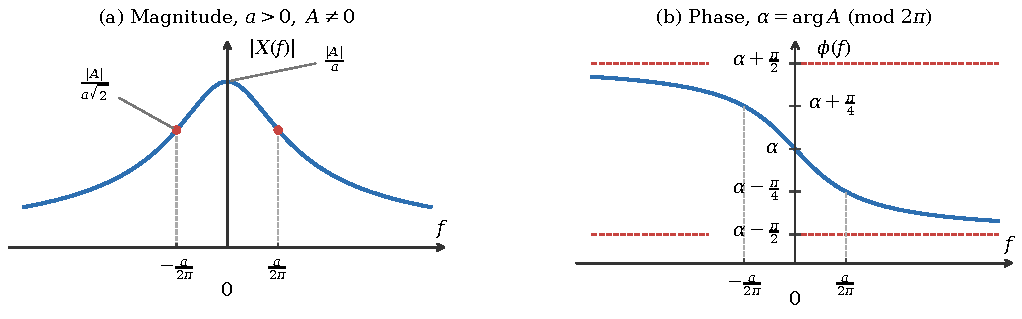
\includegraphics[width=.98\linewidth]{hw02-exponential.pdf}
\end{center}


\subsection*{本题知识点与公式}
\label{kn:2-2}
\begin{focusbox}{已学前置与本题新增}
强度、能量和频率单位见第\ref{kn:2-1}题。本题首次建立复数幅相、傅里叶变换、实信号频谱对称性以及时间尺度与谱宽的关系。后续的频移、调制和系统频响都使用这些约定。
\end{focusbox}

\subsubsection*{1. 复数的幅值与相位：频谱计算的基本工具}
用 $\iu^2=-1$，将复数写成直角坐标与极坐标形式
\[
z=p+\iu q=|z|e^{\iu\phi},\quad |z|=\sqrt{p^2+q^2},\quad
\phi=\operatorname{atan2}(q,p),\quad z^*=p-\iu q.
\]
双参数反正切保留象限；只用 $\arctan(q/p)$ 会把 $p<0$ 的象限弄错。$z=0$ 时相位无定义，非零复数的相位相差 $2\pi k$ 表示同一点。
\[
|z_1z_2|=|z_1||z_2|,\quad
\arg(z_1z_2)=\arg z_1+\arg z_2,
\]
\[
\left|\frac{z_1}{z_2}\right|=\frac{|z_1|}{|z_2|},\quad
\arg\frac{z_1}{z_2}=\arg z_1-\arg z_2\qquad(z_2\ne0).
\]
乘除运算可对模相乘除、相位相加减；加减运算却须先合并实虚部。通常 $|z_1+z_2|\ne|z_1|+|z_2|$，这正是第4、5题不能把两个幅谱直接相加的原因。

欧拉公式把振荡与复指数联系起来：
\[
e^{\iu\theta}=\cos\theta+\iu\sin\theta,\quad
\cos\theta=\frac{e^{\iu\theta}+e^{-\iu\theta}}2,\quad
\sin\theta=\frac{e^{\iu\theta}-e^{-\iu\theta}}{2\iu}.
\]
复指数 $e^{(\sigma+\iu\omega)t}$ 中，$\sigma$ 决定包络的增长/衰减，$\omega$ 决定振荡；两者都必须使指数的整体无量纲。

\subsubsection*{2. 傅里叶变换描述的是频率组成}
以 Hz 为变量的变换和反变换为
\[
X(f)=\int_{-\infty}^{\infty}x(t)e^{-\iu2\pi ft}\diff t,
\qquad x(t)=\int_{-\infty}^{\infty}X(f)e^{\iu2\pi ft}\diff f.
\]
幅谱 $|X(f)|$ 与相谱 $\arg X(f)$ 共同决定信号；一般不能只保留幅谱就重建原波形。对普通非周期可积信号，$X(f)$ 是连续频谱密度：若 $x$ 的单位为 V，则 $X(f)$ 的单位为 $\mathrm{V\,s}$，不是单个正弦的峰值电压。

$\int|x(t)|\diff t<\infty$ 是普通变换存在的常用充分条件，并非必要条件；在合适的分段光滑等条件下，反变换在连续点给出原值，在跳变点给出左右极限的平均值。若 $X$ 不绝对可积，反变换积分按对称截断极限 $\lim_{F\to\infty}\int_{-F}^{F}$ 理解。本题在 $t=0$ 有跳变，反演得到 $A/2$，而原题端点取 $A$；这个单点差异不改变频谱。常数、无限长正弦和阶跃不满足绝对可积条件，需要下一题的广义变换。

若以角频率 $\Omega$ 为变量，则
\[
X_\Omega(\Omega)=\int x(t)e^{-\iu\Omega t}\diff t=X\!\left(\frac\Omega{2\pi}\right),\qquad
x(t)=\frac1{2\pi}\int X_\Omega(\Omega)e^{\iu\Omega t}\diff\Omega.
\]
同一频率位置的连续谱数值只是换横坐标，反变换测度却有 $\diff\Omega=2\pi\diff f$。冲激谱还需结合冲激缩放律，不能只替换箭头位置；该点在第\ref{kn:2-3}题正式说明。

\subsubsection*{3. 首次用到的基本性质与检查方法}
下列等式默认变换以 $f$ 为变量，且信号满足普通或相应广义变换条件：
\begin{align*}
c_1x_1(t)+c_2x_2(t)&\longleftrightarrow c_1X_1(f)+c_2X_2(f),&&\text{线性},\\
x(t-t_d)&\longleftrightarrow X(f)e^{-\iu2\pi ft_d},&&\text{时移},\\
x(bt)&\longleftrightarrow\frac1{|b|}X\!\left(\frac fb\right),\ b\ne0,&&\text{时标伸缩},\\
x^*(t)&\longleftrightarrow X^*(-f),&&\text{共轭}.
\end{align*}
线性使复杂信号可拆成基本信号；时移仅改变相位，不改变幅谱；时间压缩会使频谱展宽，并改变谱密度的高度。若积分有意义，$X(0)=\int x(t)\diff t$，零频值可用时域面积核查；本题应为 $A/a$。

实信号满足共轭对称 $X(-f)=X^*(f)$：实部为偶函数、虚部为奇函数，幅谱为偶函数，相位可按模 $2\pi$ 取反。实偶信号的频谱为实偶函数，实奇信号的频谱为纯虚奇函数；相位不是简单地等于“虚部”。本题当 $A$ 为实数时适用这些实信号结论；若 $A$ 为一般复数，不能直接强加共轭对称。

对有限能量信号，帕塞瓦尔关系为（普通变换不收敛时，$X$ 按均方意义定义）
\[
\int|x(t)|^2\diff t=\int|X(f)|^2\diff f
=\frac1{2\pi}\int|X_\Omega(\Omega)|^2\diff\Omega.
\]
它连接时域能量与频域能量，$|X|^2$ 是能量谱密度，不是周期功率信号中冲激频谱的平方。

\subsubsection*{4. 单边指数的时间尺度与频谱特征}
因 $t<0$ 为零，本题应写 $Ae^{-at}u(t)$，其中 $a$ 的单位是 $\mathrm{s^{-1}}$。时间常数 $\tau_e=1/a$ 表示指数包络在 $t=\tau_e$ 时降至初值的 $e^{-1}$。由答案
\[
\frac{|X(f)|}{|X(0)|}=\frac1{\sqrt{1+(2\pi f/a)^2}},\quad
f_b=\frac a{2\pi},\quad E_x=\frac{|A|^2}{2a}.
\]
$f_b$ 处幅值为零频值的 $1/\sqrt2$，幅值平方为一半；在很高频率下 $|X(f)|\sim|A|/(2\pi|f|)$。$a$ 增大使衰减更快、归一化频谱更宽，但零频高度 $|A|/a$ 更低。此结论描述同一信号的时频对应，尚不等于已经给定某个测量系统的传递函数。


\nt{
    \textbf{易错：单边指数信号的负时间区间为零；横轴单位必须统一。}
    若去掉 $u(t)$，把 $Ae^{-at}$ 定义在全时间轴上，
    它在 $t\to-\infty$ 时发散，
    上述普通傅里叶积分不成立。
    用谱角频率写时为 $A/(a+\iu\Omega)$，
    改用 $f$ 后必须代入 $\Omega=2\pi f$。
    当 $A$ 为负实数时，可取 $\alpha=\pi$，再按所需主值区间折回相位；
    $A=0$ 时相位没有定义。
}

\needspace{11\baselineskip}
\section{第3题：符号函数与单位阶跃函数的广义频谱}
\label{hw:2-3}
\keypoint{复习重点：微分性质、冲激项、主值分布及其谱图表示。}

\begin{hwquestion}
求 $\sgn(t)$ 与 $u(t)$ 的频谱，
    使用频率 $f$ 为横坐标绘制幅频图与相频图。
    采用 $\sgn(0)=0$、$u(0)=1/2$ 的对称约定。
\end{hwquestion}

\subsection*{答案与解析}
这两个信号不绝对可积，不能把普通积分当作收敛积分计算。
引入主值符号 $\PV$，用对称方式处理 $f=0$ 附近的奇性。
\textbf{以下变换等式在广义函数意义下成立。}

\subsubsection{符号函数：用微分性质确定连续部分}
\[
    \sgn(t)=
    \begin{cases}
        -1,&t<0,\\
        1,&t>0,
    \end{cases}
    \qquad
    \frac{\diff}{\diff t}\sgn(t)=2\delta(t).
\]
设 $S(f)=\mathcal F\{\sgn(t)\}$。由
$\mathcal F\{x'(t)\}=\iu2\pi fX(f)$、
$\mathcal F\{\delta(t)\}=1$ 得
\[
    \iu2\pi fS(f)=2.
\]
在 $f\neq0$ 时，$S(f)=1/(\iu\pi f)$。
微分式本身不能排除 $C\delta(f)$，因为 $f\delta(f)=0$；
但 $\sgn(t)$ 是实奇函数，其频谱必须为纯虚奇分布，
不能含偶的 $\delta(f)$ 项。因此
\[
    \boxed{\mathcal F\{\sgn(t)\}
    =\PV\!\left(\frac{1}{\iu\pi f}\right)}.
\]
也可用收敛信号验证这个结果。令
$s_\varepsilon(t)=\sgn(t)e^{-\varepsilon|t|}$，$\varepsilon>0$，则
\begin{align*}
    \mathcal F\{s_\varepsilon(t)\}
    &=\frac{1}{\varepsilon+\iu2\pi f}
      -\frac{1}{\varepsilon-\iu2\pi f} \\
    &=\frac{-\iu4\pi f}{\varepsilon^2+(2\pi f)^2}
      \xrightarrow[\varepsilon\downarrow0]{\text{广义极限}}
      \PV\!\left(\frac{1}{\iu\pi f}\right).
\end{align*}

\subsubsection{单位阶跃：由符号函数补齐零频冲激}
利用 $u(t)=[1+\sgn(t)]/2$ 与 $\mathcal F\{1\}=\delta(f)$，可得
\[
    \boxed{U(f)=\mathcal F\{u(t)\}
    =\frac12\delta(f)
      +\PV\!\left(\frac{1}{\iu2\pi f}\right)}.
\]
这里 $\delta(f)/2$ 来自阶跃的常值分量。
若只对 $u'(t)=\delta(t)$ 做变换，
得到 $\iu2\pi fU(f)=1$，会漏掉微分消去的零频项；
所以必须另外确定冲激的系数。

\subsubsection{如何画幅频与相频示意图}
对 $f\neq0$，频谱是通常的复数函数，因而可以写
\[
    |S(f)|=\frac{1}{\pi|f|},
    \qquad
    |U_{\mathrm c}(f)|=\frac{1}{2\pi|f|},
\]
其中 $U_{\mathrm c}$ 表示阶跃谱的连续部分。两者相位相同：
\[
    \phi(f)=
    \begin{cases}
        +\pi/2,&f<0,\\
        -\pi/2,&f>0.
    \end{cases}
\]

\begin{center}
    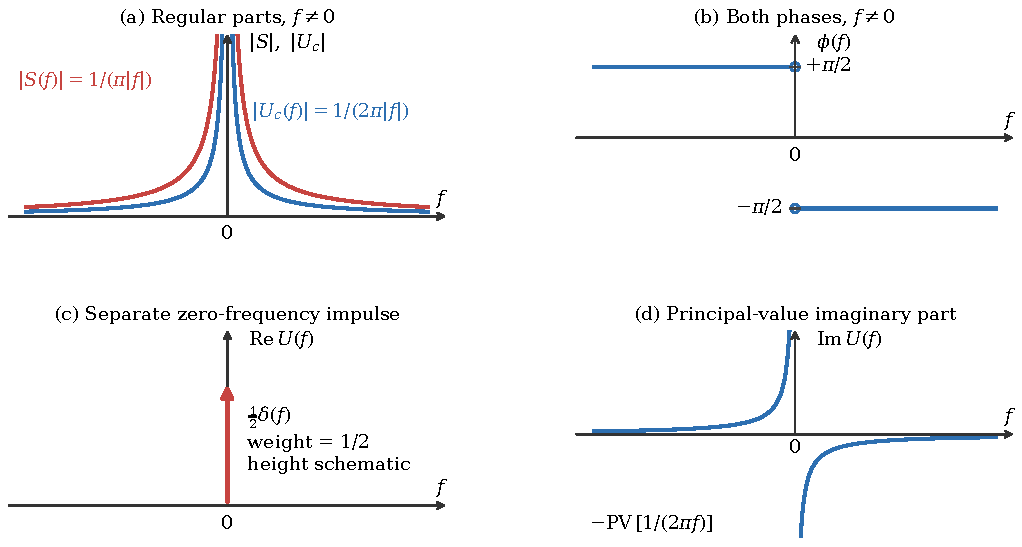
\includegraphics[width=.98\linewidth]{hw03-generalized.pdf}
\end{center}


\subsection*{本题知识点与公式}
\label{kn:2-3}
\begin{focusbox}{已学前置与本题新增}
复数幅相和变换约定见第\ref{kn:2-2}题。本题首次讲清冲激的权重、主值分布、微分/积分的变换性质，以及常数和正余弦线谱。核心是区分“普通函数在非零频率的值”与“整个广义频谱”。
\end{focusbox}

\subsubsection*{1. 单位冲激不是有限高度、零宽度的普通曲线}
冲激 $\delta(t)$ 由筛选作用定义：对适当连续的测试函数 $g$，
\[
\int_{-\infty}^{\infty}\delta(t-t_d)g(t)\diff t=g(t_d),\qquad
\int\delta(t)\diff t=1.
\]
因此 $c\delta(t-t_d)$ 的位置为 $t_d$、权重为 $c$；画谱时标注的是权重，而不是一个有限峰高。$\delta(t)$ 的量纲是 $\mathrm{s^{-1}}$，其积分才无量纲。与普通函数相乘时有
\[
g(t)\delta(t-t_d)=g(t_d)\delta(t-t_d),\qquad
t\delta(t)=0,\qquad \delta(bt)=\frac1{|b|}\delta(t)\quad(b\ne0).
\]
缩放式的绝对值来自保持积分权重不变。阶跃的广义导数为 $u'(t)=\delta(t)$；跳变大小为2的符号函数满足 $\sgn'(t)=2\delta(t)$。跳变点的单点赋值不改变这些关系。

\subsubsection*{2. 为什么要用主值，而不能直接计算 $1/f$ 在零点的值}
$1/f$ 在零点奇异，普通的左右两个反常积分均不收敛。取光滑且在无穷远快速衰减的测试函数 $g$，柯西主值采用对称删去零点附近区间后再取极限：
\[
\left\langle\PV\frac1f,g\right\rangle
=\lim_{\eta\downarrow0}\left(\int_{-\infty}^{-\eta}\frac{g(f)}f\diff f+
\int_{\eta}^{\infty}\frac{g(f)}f\diff f\right).
\]
尖括号表示分布对测试函数 $g$ 的作用。这定义了一种分布，而不是为 $f=0$ 人为指定一个数。$\PV(1/f)$ 与 $\delta(f)$ 作用方式不同：前者保留非零频率处的奇函数结构，后者只筛选零频处的信息。不能把主值奇性画成多余的冲激，也不能对含分布的整个表达式按普通复数直接取模或平方。

\subsubsection*{3. 微分性质为何不能唯一恢复零频项}
由分部积分，在端点项消失的条件下，
\[
\mathcal F\{x^{(n)}(t)\}=(\iu2\pi f)^nX(f).
\]
阶跃等信号须以广义函数意义使用。反过来求 $X$ 时，乘子 $f$ 会消去 $C\delta(f)$，所以除以 $f$ 后只能先确定非零频率部分。必须再用已知常数分量、奇偶性或原函数定义确定 $C$。本题符号函数的奇性排除偶冲激，而阶跃中的 $1/2$ 常数保留 $\delta(f)/2$。

把从负无穷积分写成与阶跃卷积，可得相应积分性质
\[
z(t)=\int_{-\infty}^{t}x(\lambda)\diff\lambda
\quad\longleftrightarrow\quad
Z(f)=\PV\frac{X(f)}{\iu2\pi f}+\frac{X(0)}2\delta(f),
\]
一个充分条件是 $x(t)$ 与 $t\,x(t)$ 都绝对可积，使 $X$ 在零点附近连续可微；等式按广义函数意义理解，不可直接对含未定义分布乘积的任意 $X$ 使用。最后一项不能随意省略；积分下限或积分常数改变，也可能改变直流冲激项。卷积的一般定义在第\ref{kn:2-4}题展开。

\subsubsection*{4. 应记住的广义变换对与正负频率相位}
在本册 Hz 约定下，$f_s>0$，有
\begin{align*}
\delta(t-t_d)&\longleftrightarrow e^{-\iu2\pi ft_d},\\
1&\longleftrightarrow\delta(f),\\
e^{\iu2\pi f_st}&\longleftrightarrow\delta(f-f_s),\\
\cos2\pi f_st&\longleftrightarrow\tfrac12[\delta(f-f_s)+\delta(f+f_s)],\\
\sin2\pi f_st&\longleftrightarrow\tfrac1{2\iu}[\delta(f-f_s)-\delta(f+f_s)].
\end{align*}
正余弦的谱线来自第\ref{kn:2-2}题的欧拉公式。正弦正频率的权重为 $-\iu/2$、负频率为 $+\iu/2$；两者的模均为 $1/2$，相位依次为 $-\pi/2$、$+\pi/2$。负频率是复指数相反的旋转方向，不是另一种独立的物理正弦。

本题两个重要变换对为
\[
\sgn(t)\longleftrightarrow\PV\frac1{\iu\pi f},\qquad
u(t)\longleftrightarrow\frac12\delta(f)+\PV\frac1{\iu2\pi f}.
\]
非零频率处均为纯虚数，$f>0$ 时为负虚数，故相位 $-\pi/2$；$f<0$ 时相位 $+\pi/2$。阶跃频谱的零频冲激需单独标注，不能把非零频率相位延伸到整个零频分布。

若改用角频率，利用 $\delta(\Omega/(2\pi)-f_s)=2\pi\delta(\Omega-2\pi f_s)$，可得
\[
\mathcal F_\Omega\{1\}=2\pi\delta(\Omega),\quad
\mathcal F_\Omega\{\cos\omega_st\}=\pi[\delta(\Omega-\omega_s)+\delta(\Omega+\omega_s)],
\]
\[
\mathcal F_\Omega\{u(t)\}=\pi\delta(\Omega)+\PV\frac1{\iu\Omega}.
\]
正是冲激缩放律使权重出现 $2\pi$；不能把 Hz 谱箭头平移到角频率横轴后仍保留原权重。


\nt{
    \textbf{易错：广义频谱不能在 $f=0$ 处直接取模。}
    图中的曲线仅表示 $f\neq0$ 的连续部分；
    阶跃谱在 $f=0$ 处还须单独画一个冲激箭头，标注\textbf{权重 $1/2$}。
    箭头长度不是有限的冲激高度，也不能把
    $|\delta(f)/2+1/(\iu2\pi f)|$ 当作普通函数计算。
    $f=0$ 的整个广义频谱不具有普通“幅值、相位”数值。
    符号函数的奇性是主值项，不能误画成额外的零频冲激。
}

\Needspace{11\baselineskip}
\section{第4题：截断余弦与两个平移的矩形窗频谱}
\label{hw:2-4}
\keypoint{复习重点：矩形窗变换、调制性质、幅频与有符号频谱的区别。}

\begin{hwquestion}
求
    \[
        y(t)=
        \begin{cases}
            \cos2\pi f_0t,&|t|\leq T,\\
            0,&|t|>T
        \end{cases}
    \]
    的傅里叶变换，并以 $f$ 为横坐标绘制频谱。
    其中 $T>0$，截断窗口总宽度为 $2T$。
\end{hwquestion}

\subsection*{答案与解析}
\textbf{先求窗谱，再搬移到 $\pm f_0$。}
令 $w(t)=1$（$|t|\leq T$），其余处为 $0$，则
$y(t)=w(t)\cos2\pi f_0t$。
\begin{align*}
    W(f)
    &=\int_{-T}^{T}e^{-\iu2\pi ft}\diff t \\
    &=\frac{e^{\iu2\pi fT}-e^{-\iu2\pi fT}}{\iu2\pi f}
      =\frac{\sin2\pi fT}{\pi f}
      =2T\Sa(2\pi fT).
\end{align*}
$f=0$ 处由极限补上 $W(0)=2T$。利用欧拉公式与频移性质：
\begin{align*}
    y(t)
    &=\frac12w(t)e^{\iu2\pi f_0t}
      +\frac12w(t)e^{-\iu2\pi f_0t},\\
    Y(f)
    &=\frac12W(f-f_0)+\frac12W(f+f_0).
\end{align*}
\[
    \boxed{Y(f)=T\Sa\bigl(2\pi T(f-f_0)\bigr)
       +T\Sa\bigl(2\pi T(f+f_0)\bigr)}.
\]
这也等价于把两条理想余弦谱线
$[\delta(f-f_0)+\delta(f+f_0)]/2$
分别与 $W(f)$ 卷积。

为绘制两个平移分量，记
\[
    Y_+(f)=T\Sa\bigl(2\pi T(f-f_0)\bigr),
    \qquad
    Y_-(f)=T\Sa\bigl(2\pi T(f+f_0)\bigr).
\]
下图分别画出 $Y_+(f)$ 和 $Y_-(f)$，竖线用于定位各自的中心频率。
$Y_+$ 在 $f=f_0$ 处峰高为 $T$，首零点为 $f_0\pm1/(2T)$；
$Y_-$ 在 $f=-f_0$ 处峰高为 $T$，首零点为 $-f_0\pm1/(2T)$。
这些峰和零点均属于\textbf{单个分量}；真正的总谱必须逐点代数相加：
$Y(f)=Y_+(f)+Y_-(f)$。

\begin{center}
    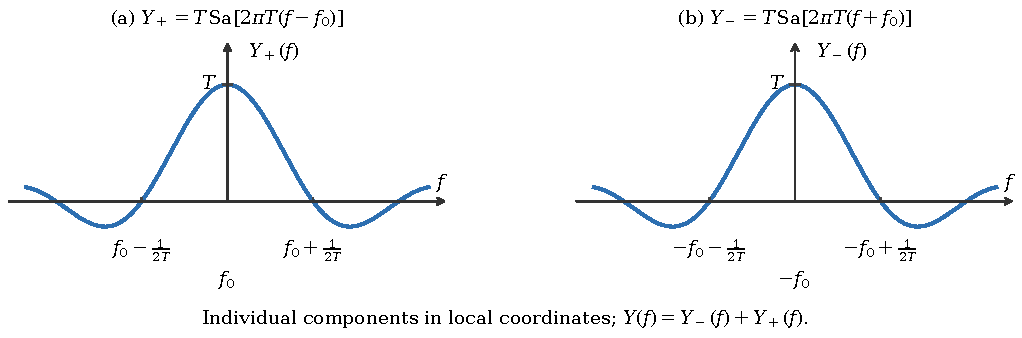
\includegraphics[width=.98\linewidth]{hw04-windowed.pdf}
\end{center}

\needspace{6\baselineskip}
\textbf{总频谱的幅值与相位。}
因为 $y(t)$ 为实偶函数，$Y(f)$ 也是实偶函数，
但其旁瓣可取负值。
幅频图应画 $|Y(f)|$；有符号的频谱图则保留负旁瓣。相位为
\[
    \phi(f)=
    \begin{cases}
        0,&Y(f)>0,\\
        \pi\quad(\mathrm{mod}\ 2\pi),&Y(f)<0,
    \end{cases}
\]
$Y(f)=0$ 处相位无定义。

\begin{center}
    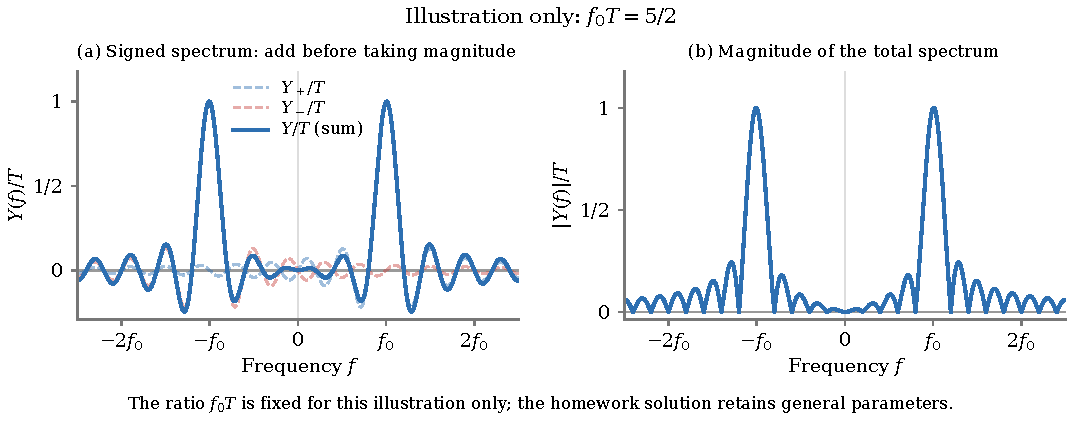
\includegraphics[width=.98\linewidth]{homework-windowed-total.pdf}
\end{center}
上图仅取 $f_0T=5/2$ 展示两个分量的代数相加与取模，未给原题增添已知条件；横轴为频率 $f$，纵轴除以 $T$ 归一化。左图保留总谱的正负旁瓣，右图为总幅谱。其他 $f_0T$ 比值的谱形由前述通式确定。


\subsection*{本题知识点与公式}
\label{kn:2-4}
\begin{focusbox}{已学前置与本题新增}
变换、复数叠加见第\ref{kn:2-2}题，余弦的冲激线谱见第\ref{kn:2-3}题。本题首次系统讲频移、卷积、时域相乘、矩形窗与主旁瓣。核心操作顺序是“构造复频谱，再相加，最后取模”。
\end{focusbox}

\subsubsection*{1. 频移性质与时移性质必须分开}
将指数乘子直接代入变换定义，可得
\[
\mathcal F\{x(t)e^{\iu2\pi f_ct}\}
=\int x(t)e^{-\iu2\pi(f-f_c)t}\diff t=X(f-f_c).
\]
所以频域的 $f-f_c$ 表示向右移动 $f_c$，$f+f_c$ 表示向左移动 $f_c$。利用欧拉公式，
\begin{align*}
x(t)\cos2\pi f_ct&\longleftrightarrow\tfrac12[X(f-f_c)+X(f+f_c)],\\
x(t)\sin2\pi f_ct&\longleftrightarrow\tfrac1{2\iu}[X(f-f_c)-X(f+f_c)].
\end{align*}
余弦为两个副本相加，正弦为复数副本相减。对照第\ref{kn:2-2}题，$x(t-t_d)$ 引入的是频域相位因子，既不搬动幅谱，也不产生这两个副本。

\subsubsection*{2. 卷积的定义、筛选作用与乘积定理}
时域卷积定义为
\[
(x*h)(t)=\int_{-\infty}^{\infty}x(\lambda)h(t-\lambda)\diff\lambda.
\]
它把各时刻 $x(\lambda)$ 对延迟响应 $h(t-\lambda)$ 的贡献累加；一般不是逐点乘积。频域卷积同理定义为
\[
(X*H)(f)=\int_{-\infty}^{\infty}X(\nu)H(f-\nu)\diff\nu.
\]
交换、结合和分配关系在适当的收敛条件下成立。冲激的筛选作用给出 $X(f)*\delta(f-f_c)=X(f-f_c)$，因而与冲激线谱卷积恰好产生频移。

在 Hz 变换约定下，两条成对性质为
\[
x(t)*h(t)\longleftrightarrow X(f)H(f),\qquad
x(t)h(t)\longleftrightarrow X(f)*H(f).
\]
第二式可把一个因子的反变换代入积分，并交换积分顺序推得。本题属于第二式：矩形窗与余弦在时域相乘，频域中窗谱与两条余弦冲激卷积。角频率约定下，时域乘积的频域卷积前须有 $1/(2\pi)$；不同约定不可混用。

\subsubsection*{3. 矩形窗、Sa与sinc的宽度约定}
记 $\operatorname{rect}(v)=1$（$|v|<1/2$），外部为零；端点定义不影响积分。若观察总时长为 $L$，则
\[
w_L(t)=\operatorname{rect}\!\left(\frac tL\right),\qquad
W_L(f)=L\Sa(\pi Lf)=L\operatorname{sinc}(Lf),
\]
其中 $\Sa z=\sin z/z$，归一化 $\operatorname{sinc}v=\sin(\pi v)/(\pi v)$，两者的自变量不同。$W_L(0)=L$，非零零点为 $f=k/L$（整数 $k\ne0$）。中心两侧首零点为 $\pm1/L$，主瓣零点间宽度为 $2/L$；其余振荡瓣称旁瓣。

本题 $L=2T$，所以 $W(f)=2T\Sa(2\pi Tf)$。乘以余弦后，两个副本各乘 $1/2$，分别以 $\pm f_0$ 为中心；各自的峰高 $T$、首零点偏移 $1/(2T)$、主瓣宽度 $1/T$ 都由此得出。它们是\textbf{各个分量}的属性，不保证就是总谱的峰高、峰位和零点。总谱仍满足
\[
Y(0)=2T\Sa(2\pi f_0T),\qquad
Y(f_0)=T[1+\Sa(4\pi f_0T)].
\]

\subsubsection*{4. 为什么截断产生泄漏，延长观察时间有什么作用}
无限长余弦的全部频率组成集中于 $\pm f_0$ 两条线；有限时长观察相当于加窗，窗谱把每条线展宽，并产生延伸到远处的旁瓣，这叫频谱泄漏。矩形窗的尾部只按约 $1/|f|$ 衰减，因而严格时限不等于严格带限。

增大 $L$ 会使首零点间距缩小，改善区分相近频率成分的能力；同时连续谱密度的峰高随 $L$ 增长，不能把这个增长误认为原余弦的时域峰值改变。窗函数的主瓣宽度与旁瓣大小存在折中：平滑端点通常能降低远旁瓣，却会改变主瓣宽度，具体指标应由所用窗计算，不能沿用矩形窗的零点公式。

本题的实偶时域信号使总谱为实偶，但负旁瓣仍代表相位 $\pi$；画有符号谱保留负值，画幅谱才取绝对值。先把旁瓣绝对化再叠加，会失去相消与相位信息，得到另一幅错误的谱。


\nt{
    \textbf{易错：截断并未保留两条理想谱线。}
    时域相乘对应频域卷积，有限窗口把谱线展宽为带旁瓣的连续谱。
    $T$ 是半窗宽，窗口频谱为 $2T\Sa(2\pi fT)$，
    不能误写成 $T\Sa(\pi fT)$。
    窗越长，主瓣越窄；两个平移的窗谱需要先做\textbf{代数相加}，
    再取绝对值，不能把两个窗谱的模直接相加。
    两端点取不取等号不影响傅里叶积分。
}

\needspace{11\baselineskip}
\section{第5题：指数衰减振荡的频谱与实际峰位}
\label{hw:2-5}
\keypoint{复习重点：指数谱频移、复数合并与幅频峰的位置。}

\begin{hwquestion}
原题为 $x(t)=e^{-at}\sin\omega t$。结合第2题，按 $a>0$、$\omega>0$ 且 $t\geq0$ 的单边衰减振荡解释，即
    $x(t)=e^{-at}\sin\omega t\,u(t)$。
    利用单边指数信号的频谱及傅里叶变换性质，求其频谱，
    并以 $f$ 为横坐标绘制幅频图。
\end{hwquestion}

\subsection*{答案与解析}
令 $g(t)=e^{-at}u(t)$，单边指数信号的变换为
$G(f)=1/(a+\iu2\pi f)$。
设振荡频率 $f_{\mathrm s}=\omega/(2\pi)$，由
$\sin\omega t=(e^{\iu\omega t}-e^{-\iu\omega t})/(2\iu)$ 得
\begin{align*}
    X(f)
    &=\frac{1}{2\iu}\bigl[G(f-f_{\mathrm s})-G(f+f_{\mathrm s})\bigr]\\
    &=\frac{1}{2\iu}
      \left[
        \frac{1}{a+\iu(2\pi f-\omega)}
        -\frac{1}{a+\iu(2\pi f+\omega)}
      \right]\\
    &=\boxed{\frac{\omega}{(a+\iu2\pi f)^2+\omega^2}}.
\end{align*}
把分母分成实部和虚部，得到幅频表达式
\[
    \boxed{
    |X(f)|=
    \frac{\omega}
    {\sqrt{\bigl[a^2+\omega^2-(2\pi f)^2\bigr]^2
    +4a^2(2\pi f)^2}}
    }.
\]
该幅值是偶函数，零频处为
$|X(0)|=\omega/(a^2+\omega^2)$。

\subsubsection*{幅谱峰位的推导}
令 $q=(2\pi f)^2\geq0$。幅值最大等价于其分母平方最小：
\begin{align*}
    D(q)
    &=(a^2+\omega^2-q)^2+4a^2q\\
    &=q^2+2(a^2-\omega^2)q+(a^2+\omega^2)^2,\\
    D'(q)&=2(q+a^2-\omega^2).
\end{align*}
因此，
\[
    \boxed{
    f_{\mathrm{peak}}=
    \begin{cases}
        \displaystyle\pm\frac{\sqrt{\omega^2-a^2}}{2\pi},
            &\omega>a,\\[2mm]
        0,&0<\omega\leq a.
    \end{cases}}
\]
当 $\omega>a$ 时，存在两个对称峰，峰高为 $1/(2a)$；
当 $\omega\leq a$ 时，最大值在中心，峰高为
$\omega/(a^2+\omega^2)$。
弱衰减 $a\ll\omega$ 时，双峰才接近 $\pm\omega/(2\pi)$。


绘制幅谱时，先标出中心值 $\omega/(a^2+\omega^2)$、上述峰位和峰高，
再利用关于纵轴的对称性补齐曲线。
下图分别示意 $\omega>a$ 的双峰与 $0<\omega\leq a$ 的中心单峰。

\begin{center}
    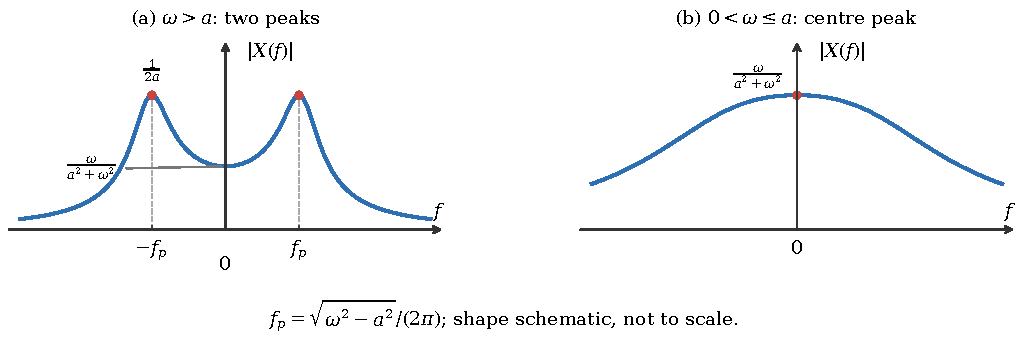
\includegraphics[width=.98\linewidth]{hw05-damped.pdf}
\end{center}


\subsection*{本题知识点与公式}
\label{kn:2-5}
\begin{focusbox}{已学前置与本题新增}
指数谱见第\ref{kn:2-2}题，正弦线谱和频移见第\ref{kn:2-3}、\ref{kn:2-4}题。本题新增单边阻尼振荡的包络、谱相位、能量，以及“振荡频率”和“幅谱峰位”之间的区别；变换性质本身不再重复推导。
\end{focusbox}

\subsubsection*{1. 衰减率与振荡频率控制不同的时间特征}
对 $e^{-at}\sin\omega t\,u(t)$，$a>0$ 的单位为 $\mathrm{s^{-1}}$，$\omega>0$ 的单位为 $\mathrm{rad/s}$。指数包络为 $\pm e^{-at}$，包络时间常数为 $1/a$；正弦因子的振荡周期为 $T_s=2\pi/\omega$，每经过一个振荡周期，包络比值为
\[
\frac{e^{-a(t+T_s)}}{e^{-at}}=e^{-2\pi a/\omega}.
\]
因此 $a/\omega$ 是判断衰减相对振荡快慢的无量纲量。整个信号不是周期信号，尽管其中的正弦因子有周期。乘上 $u(t)$ 又破坏了整条时间轴上的奇对称，不能因为含正弦便断言其频谱纯虚。

\subsubsection*{2. 两个复数副本相减后，幅值与相位怎样提取}
第\ref{kn:2-4}题的正弦调制公式给出两个指数谱的差；合并后设
\[
X(f)=\frac{\omega}{D_R(f)+\iu D_I(f)},\quad
D_R=a^2+\omega^2-(2\pi f)^2,\quad D_I=4\pi af.
\]
由于分子为正实数，相位为
\[
\phi(f)=-\operatorname{atan2}\!\left(4\pi af, a^2+\omega^2-(2\pi f)^2\right).
\]
零频处相位为零；当正频率足够大时，分母实部为负、虚部为正，输出相位趋于 $-\pi$，不能用普通反正切误画成回到零。负频率相位按共轭对称取反；幅谱始终为偶函数。这里 $X(f)$ 没有有限频率零点，因为 $\omega>0$ 且分母对实 $f$ 不为零。

谱峰位置由分母模的极小值决定，不能只看频移中心。答案已经给出 $\omega>a$ 时的双峰 $\pm\sqrt{\omega^2-a^2}/(2\pi)$ 与 $\omega\leq a$ 时的中心峰。弱衰减条件下可展开为
\[
f_{\mathrm{peak},+}=\frac{\omega}{2\pi}\sqrt{1-\frac{a^2}{\omega^2}}
\approx\frac{\omega}{2\pi}\left(1-\frac{a^2}{2\omega^2}\right),\qquad a/\omega\ll1.
\]
这个近似说明峰位接近正弦频率需要额外条件，不是频移公式自动保证的结论。

\subsubsection*{3. 用能量和高频渐近检查频谱}
由 $\sin^2\omega t=(1-\cos2\omega t)/2$ 及指数积分，
\begin{align*}
E_x&=\int_0^\infty e^{-2at}\sin^2\omega t\diff t\\
&=\frac1{4a}-\frac{a}{4(a^2+\omega^2)}
=\frac{\omega^2}{4a(a^2+\omega^2)}.
\end{align*}
本题是有限能量信号，平均功率为零，帕塞瓦尔关系可据此检查 $\int|X(f)|^2\diff f$。在 $|f|\to\infty$ 时，
\[
|X(f)|\sim\frac{\omega}{(2\pi f)^2}.
\]
其高频衰减比第2题的 $1/|f|$ 更快：本题在 $t=0$ 连续且为零，而单边指数在零点有幅值跳变；时域边界的光滑性会影响频域尾部。不能据此取消本题的单边条件，也不能把它替换为双边 $e^{-a|t|}\sin\omega t$，那是另一个信号。

\nt{
    \textbf{易错：两次频移后的复数谱要先相减，再取模。}
    不能把 $|X(f)|$ 画成两个指数幅频图的简单叠加，
    也不能因正弦的名义频率是 $\omega$ 就把最大值固定在 $\pm\omega$。
    这里横轴为 $f$，频率位置均须除以 $2\pi$。
    若省略 $u(t)$ 而把原式定义在整条实轴上，
    负时间方向会指数增长，普通傅里叶积分不收敛。
}

\needspace{11\baselineskip}
\section{第6题：余弦调制与频谱搬移、重叠}
\label{hw:2-6}
\keypoint{复习重点：欧拉展开的 $1/2$ 系数、两个搬移副本及频带重叠条件。}

\begin{hwquestion}
原题中的时间函数记作 $f(t)$。为避免与频率变量 $f$ 混淆，以下将其改记为 $m(t)$，频谱为 $M(f)$，按原图采用实值带限模型
    \[
        M(f)=0\quad(|f|>f_m),
        \qquad f_m=\frac{\omega_m}{2\pi}>0.
    \]
    采用角频率为 $\omega_0>0$ 的余弦载波，记
    \[
        f_{\mathrm c}=\frac{\omega_0}{2\pi},
        \qquad s(t)=m(t)\cos\omega_0t.
    \]
    求调幅信号 $s(t)$ 的傅里叶变换，示意画出时域和频域信号，
    并讨论 $\omega_0>\omega_m$、$\omega_0=\omega_m$
    与 $\omega_0<\omega_m$ 时的频带关系。
\end{hwquestion}

\subsection*{答案与解析}
利用欧拉公式展开载波，再应用频移性质：
\begin{align*}
    s(t)
    &=\frac12m(t)e^{\iu2\pi f_{\mathrm c}t}
      +\frac12m(t)e^{-\iu2\pi f_{\mathrm c}t}.
\end{align*}
\[
    \boxed{S(f)=\frac12M(f-f_{\mathrm c})
        +\frac12M(f+f_{\mathrm c})}.
\]
两项分别把原谱搬到正、负载频处，
每个副本都乘 $1/2$，谱形保持不变。
若改用谱角频率 $\Omega$ 为横轴，定义
$\mathcal M(\Omega)=M(\Omega/2\pi)$、
$\mathcal S(\Omega)=S(\Omega/2\pi)$，则同一结论写作
\[
    \boxed{\mathcal S(\Omega)
      =\frac12\mathcal M(\Omega-\omega_0)
       +\frac12\mathcal M(\Omega+\omega_0)}.
\]

\subsubsection{时域图：快速振荡受调制信号控制}
对于实信号，$|s(t)|\leq|m(t)|$ 始终成立。
在本题严格带限且 $f_c>f_m$ 的谱分离条件下，可先画 $m(t)$ 的形状，再在其内部画载波振荡，解析幅值包络为 $|m(t)|$；若 $m(t)\geq0$，上下包络为 $\pm m(t)$。$m(t)$ 变号时还会使载波翻转 $\pi$ 相位。若载频过低、两谱副本重叠，则 $\pm|m(t)|$ 仍提供逐点幅值界，但一般不再等于解析包络。
该调制信号没有额外的常值载波项，
是双边带抑制载波调制的基本形式。

下图根据给定的 $m(t)$ 轮廓，在包络内画出载波振荡，
并将一般的 $M(f)$ 轮廓左右平移以构造调制频谱。
时域包络与频谱轮廓为形状示意；
频带端点和每个副本的 $1/2$ 系数由变换公式决定。

\begin{center}
    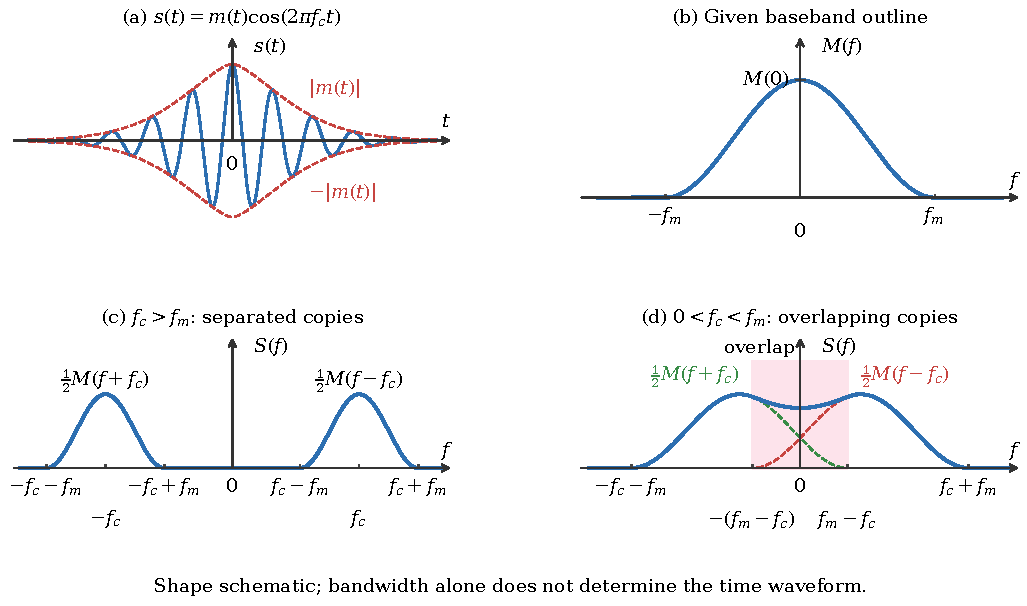
\includegraphics[width=.98\linewidth]{hw06-modulation.pdf}
\end{center}


\subsection*{本题知识点与公式}
\label{kn:2-6}
\begin{focusbox}{已学前置与本题新增}
频移和卷积见第\ref{kn:2-4}题，冲激线谱见第\ref{kn:2-3}题。本题新增基带、载波、边带和带宽的完整含义，频带重叠与相干解调，并补齐后续多频应变和调幅题需要的傅里叶级数与谱线幅值约定。
\end{focusbox}

\subsubsection*{1. 基带、载波、边带及带宽应怎样定义}
$m(t)$ 携带被测信息，称调制信号，其未经搬移的频谱称基带谱；$\cos2\pi f_ct$ 为载波，$s(t)$ 为已调信号。本题是乘法调制：信息改变高频振荡的幅值及正负符号。严格带限模型 $M(f)=0$（$|f|>f_m$）中，$f_m$ 为基带最高频率；基带正频率带宽为 $f_m$，不要把双边支撑区间的宽度 $2f_m$ 也叫同一个基带带宽。

调制的两个副本支撑在
\[
I_+=[f_c-f_m,f_c+f_m],\qquad I_-=[-f_c-f_m,-f_c+f_m].
\]
当 $f_c>f_m$，正载频附近的双边带占用宽度为 $B=2f_m$，上下边带分别位于载频两侧。两个副本间隔为 $2(f_c-f_m)$；$f_c=f_m$ 时在零频相接；$0<f_c<f_m$ 时交集为
\[
I_+\cap I_-=[-(f_m-f_c),\ f_m-f_c],
\]
重叠宽度 $2(f_m-f_c)$。若原谱内部有空隙或端点为零，上述区间只是可能支撑的范围；发生实际相加仍取决于两个副本在该频率处是否非零。实际非严格带限信号只能按规定的有效带宽作近似判断。

\subsubsection*{2. 抑制载波、包络与有符号信息}
本题 $s=m\cos2\pi f_ct$ 没有额外的常值载波项，称双边带抑制载波调制。若 $m$ 自身含直流 $D$，则 $D\cos2\pi f_ct$ 仍会产生载波线，不能仅凭写成乘积就断言载波处一定无线谱。对一般连续基带谱，频移也不凭空产生独立冲激。

在上述严格带限且 $f_c>f_m$ 的条件下，幅值包络为 $|m(t)|$；若 $m$ 变号，载波还翻转 $\pi$ 相位。对实际有效带限、载波远快于包络的情况，这可作近似解释。只测包络会丢失这个符号。带直流偏置的常规调幅 $[D+m(t)]\cos2\pi f_ct$ 可在频谱分离、$D+m(t)$ 不变号时用包络恢复偏置后的信号；具体多音条件在第\ref{kn:5-3}题展开。

\subsubsection*{3. 同步相乘为什么能把信息搬回低频}
将 $s(t)$ 乘同频参考 $\cos(2\pi f_ct+\theta_r)$，积化和差给出
\[
s(t)\cos(2\pi f_ct+\theta_r)
=\frac12m(t)\cos\theta_r+
\frac12m(t)\cos(4\pi f_ct+\theta_r).
\]
第一项回到基带，第二项移至 $2f_c$ 附近。低通滤波是保留低频、抑制高频的操作；若其通带覆盖 $|f|\leq f_m$，又能抑制 $2f_c$ 附近的项，则输出为 $m(t)\cos\theta_r/2$。同相时乘2可恢复原信号；相差 $90^\circ$ 时理想基带输出为零，故参考的频率与相位都重要。

$f_c>f_m$ 保证基带上端 $f_m$ 低于高频项下端 $2f_c-f_m$，为理想滤波分离提供空隙。若两个搬移副本重叠，同一变换公式仍成立，但简单带通分离以及上述直接低通恢复条件可能失效；这与离散采样造成的混叠不是同一个操作，也不等于在附加信息下任何方法都无法恢复。

\subsubsection*{4. 周期多频信号：傅里叶级数与三角系数}
后续应变和调幅题常给出多个正弦之和。对周期为 $T_0$、基角频率 $\omega_0=2\pi/T_0$ 的实信号，采用常数项直接记作 $a_0$ 的约定：
\[
x(t)=a_0+\sum_{n=1}^\infty[a_n\cos n\omega_0t+b_n\sin n\omega_0t],
\]
\[
a_0=\frac1{T_0}\int_{t_*}^{t_*+T_0}x(t)\diff t,\quad
a_n=\frac2{T_0}\int_{t_*}^{t_*+T_0}x(t)\cos n\omega_0t\diff t,
\]
\[
b_n=\frac2{T_0}\int_{t_*}^{t_*+T_0}x(t)\sin n\omega_0t\diff t.
\]
这些系数来自不同整数次正弦、余弦在一个周期上的正交性。例如对正整数 $n,m$，
\[
\int_{t_*}^{t_*+T_0}\cos n\omega_0t\cos m\omega_0t\diff t
=\begin{cases}0,&n\ne m,\\T_0/2,&n=m.\end{cases}
\]
正弦与正弦同理，正弦与余弦的交叉积分为零。将展开式乘某一基函数再积分，只留下对应项，所以非零频率系数前有 $2/T_0$。另一常见写法把常数项记作 $a_0/2$，此时常数系数定义相应改变，不能混用。分段光滑等充分条件下，级数在连续点收敛到原值，在跳变点收敛到左右极限平均值。

三角项可合并为单个余弦：
\[
a_n\cos n\omega_0t+b_n\sin n\omega_0t
=A_n\cos(n\omega_0t-\theta_n),
\]
\[
A_n=\sqrt{a_n^2+b_n^2},\qquad \theta_n=\operatorname{atan2}(b_n,a_n).
\]
若 $A_n=0$，该项相位不定义。实偶信号使 $b_n=0$，实奇信号使 $a_0=a_n=0$，可在积分前简化计算。

\subsubsection*{5. 复指数系数、单边峰值与双边冲激权重}
同一周期信号还可写为
\[
x(t)=\sum_{n=-\infty}^{\infty}C_ne^{\iu n\omega_0t},\qquad
C_n=\frac1{T_0}\int_{t_*}^{t_*+T_0}x(t)e^{-\iu n\omega_0t}\diff t.
\]
对实信号，$C_0=a_0$，$C_n=(a_n-\iu b_n)/2$（$n>0$），$C_{-n}=C_n^*$，故 $|C_{\pm n}|=A_n/2$。$C_n$ 与 $x$ 同单位；Hz 傅里叶变换为
\[
X(f)=\sum_n C_n\delta(f-nf_0),\qquad f_0=1/T_0.
\]
因此“时域余弦峰值”“复指数系数模”“角频率变换中的冲激权重的模”依次为 $A_n$、$A_n/2$、$\pi A_n$。对上式的 $A_n\cos(n\omega_0t-\theta_n)$，正角频率处实际复权重为 $2\pi C_n=\pi A_ne^{-\iu\theta_n}$，负频率处为其共轭；不能遗漏相位。这里的 $2\pi$ 来自第\ref{kn:2-3}题的冲激缩放。直流只在零频出现，不能也按正负频率分成两半。

一周期平方可积时，正交性还给出周期功率的帕塞瓦尔关系
\[
x_{\mathrm{rms}}^2=P_x=\sum_{n=-\infty}^{\infty}|C_n|^2
=a_0^2+\frac12\sum_{n=1}^\infty(a_n^2+b_n^2).
\]
它与第\ref{kn:2-1}题的有效值相连，便于计算多频信号的强度；频率不同、在共同周期正交的分量，均方值可以相加，峰值一般不能这样相加。对无限长周期信号，不应通过把冲激傅里叶谱直接平方来计算功率。


\nt{
    \textbf{易错：重叠区仍按同一变换公式计算，且系数始终为 $1/2$。}
    $\omega_0<\omega_m$ 不会使频移性质失效，
    只是两个副本在同一频率处发生叠加。
    “不能靠带通分离副本”也不等于“任何方法都无法恢复原信号”；
    恢复能力还取决于所用方法及信号的额外信息。
    时域相乘引起频域搬移，时域平移则引起相位因子，二者不可混用。
}
